	\documentclass[]{report}
\usepackage{tikz}
\newcommand{\inputtikz}[2]{%  
	\scalebox{#1}{\input{#2}}  
}
\usepackage[french]{babel}
\usepackage[utf8x]{inputenc}
\usepackage{amsmath}
\usepackage{graphicx}
%\usepackage[colorinlistoftodos]{todonotestfa}
\usepackage{listings}
\usepackage{color}
\usepackage{amsmath}
\usepackage{amsfonts}
\usepackage{mathtools}
\usepackage{graphicx}
\usepackage{caption}
\definecolor{dkgreen}{rgb}{0,0.6,0}
\definecolor{gray}{rgb}{0.5,0.5,0.5}
\definecolor{mauve}{rgb}{0.58,0,0.82}
%opening

\lstset
{frame=tb,
	language=R,
	aboveskip=3mm,
	belowskip=3mm,
	showstringspaces=false,
	framexleftmargin=5mm,
	columns= fixed,
	numbers = left,
	basicstyle={\small\ttfamily},	
	numberstyle=\tiny\color{gray},
	keywordstyle=\color{blue},
	commentstyle=\color{dkgreen},
	stringstyle=\color{mauve},
	breaklines=true,
	breakatwhitespace=true,
	tabsize=3
}

\begin{document}
	
\begin{titlepage}
	
	\newcommand{\HRule}{\rule{\linewidth}{0.5mm}} 
	
	\center 
	
	\textsc{\LARGE Université de Technologie de Compiegne}\\[1.5cm]
	\textsc{\Large SY09}\\[0.5cm] 
	\textsc{\large Data Mining}\\[0.5cm]
		
	\HRule \\[0.4cm]
	{ \huge \bfseries Premier Rendu}\\[0.4cm] 
	\HRule \\[1.5cm]
		
	\begin{minipage}{0.4\textwidth}
		\begin{flushleft} \large
			Oumaima \textsc{Talouka} 
		\end{flushleft}
	\end{minipage}
	~
	\begin{minipage}{0.4\textwidth}
		\begin{flushright} \large
			Zineb \textsc{SLAM} 
		\end{flushright}
	\end{minipage}\\[2cm]

	{\large \today}\\[2cm] 

	
\includegraphics[width=40mm]{Figures/utc.jpg}\\ % 

	\vfill
	
\end{titlepage}



\begin{abstract}


\end{abstract}

\tableofcontents

\chapter{Notes SY02}

\section{Description des Données}
 \subsection{Description des variables}

\begin{itemize}
	\item \textbf{Nom}
	\item \textbf{Spécialité}
	\item \textbf{Niveau}: Semestres de GX01 a GX06
	\item \textbf{Statut}: Soit l'étudiant est de l'UTC ou en semestre d'échange
	\item \textbf{dernier.diplome.obtenu}: 
	BAC, DUT, CPGE, ETRANGER SUPERIEUR, LICENCE, OTHER, NA
	\item \textbf{Note Médian:} min= 0, mean= 10.92, Max
	\item \textbf{Correcteur Médian:}
	\item \textbf{Note.final}
	\item \textbf{Correcteur.final}
	\item \textbf{Résultat}
\end{itemize}


\section{Analyse}

\subsection{A première vue}
	\begin{center}
	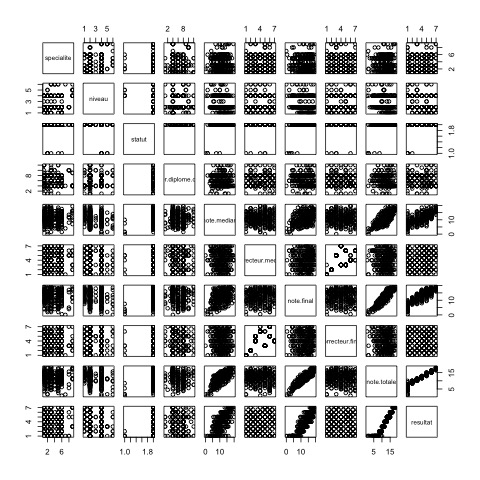
\includegraphics[width=100mm]{Figures/Notes/multiplot.jpg}
	\captionof{figure}{Plot general}
	\label{fig:multiplot_notes}
\end{center}

\subsection{Performance et homogénéité}
La figure ci-dessous représente trois diagrammes a boites des notes de médian, final et le résultat de l'UV SY02.
	\begin{center}
			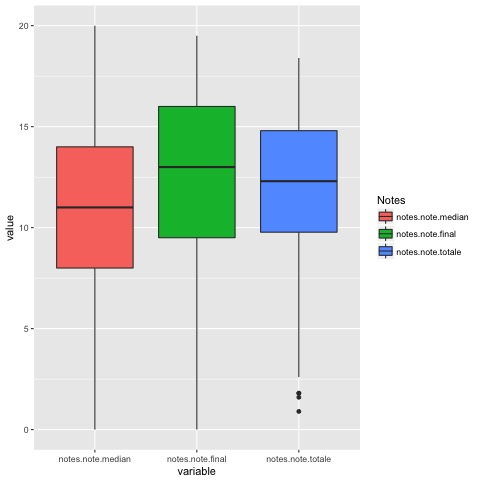
\includegraphics[width=100mm]{Figures/Notes/boxplot_exam.jpg}
			\captionof{figure}{Boxplot des Notes de Median, Final et Totale}
		    \label{fig:Boxplot_notes}
	\end{center}

On remarque que par passage du médian au final les notes ont augmente. En effet ceci est aussi témoigné par le tableau ci-dessous:

\begin{center}
	\begin{tabular}{c c c c c }
		\textbf{Notes} & \textbf{1er Quartl} & \textbf{Medianne}   & \textbf{Moyenne} & \textbf{3em Quartl} \\
		Median  & 8.0 			& 11.0		 & 10.92      & 14.0\\
		Final      & 9.50 		  & 13.0 	   & 12.38	    & 16.0\\
		Totale   & 9.775        & 12.3       &  11.845    & 14.8\\
	\end{tabular}
	\captionof{table}{Notes}
\end{center} 

Il est tout a fait logique que le digramme de résultats se situe entre les 2 puisque que c'est la moyenne \textbf{pondérée??} des 2 notes.
 
	
\subsection{Lien entre la réussite et la formation d'origine}

	\begin{center}
	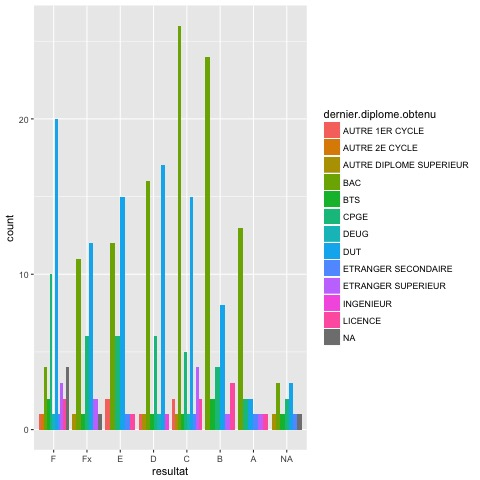
\includegraphics[width=100mm]{Figures/Notes/diplome_resultat.jpg}
	\captionof{figure}{Diagramme a baton de lien entre la formation et le resultat}
	\label{fig:formation_resultat}
	\end{center}

\subsection{Lien entre la réussite et la branche}

	\begin{center}
	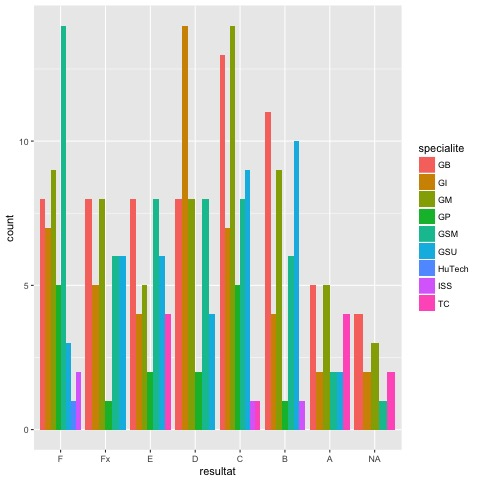
\includegraphics[width=100mm]{Figures/Notes/specialite_resultat.jpg}
	\captionof{figure}{Diagramme a baton de lien entre la branche et le resultat}
	\label{fig:specialite_resultat}
	\end{center}

\subsection{Lien entre la réussite et le niveau}

		\begin{center}
		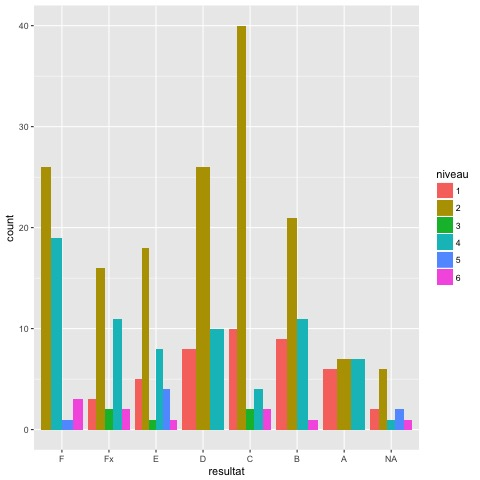
\includegraphics[width=100mm]{Figures/Notes/niveau_resultat.jpg}
		\captionof{figure}{Diagramme a baton de lien entre le niveau et le resultat}
		\label{fig:niveau_resultat}
		\end{center}

\subsection{Influence du correcteur sur la note}

	\begin{center}
	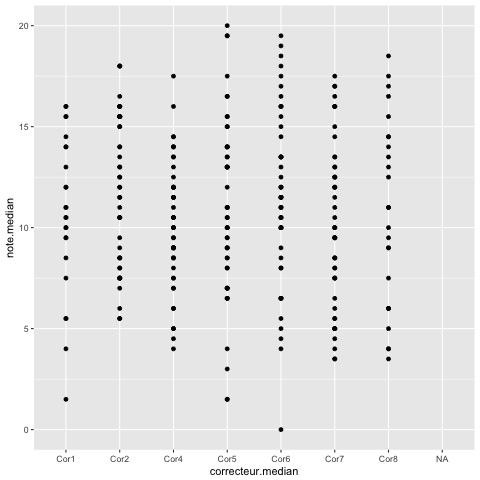
\includegraphics[width=70mm]{Figures/Notes/correcteur_median.jpg}
	\captionof{figure}{Scatterplot des notes de median en fonction des correcteurs}
	\label{fig:scatter_correcteur_median}
\end{center}

	\begin{center}
	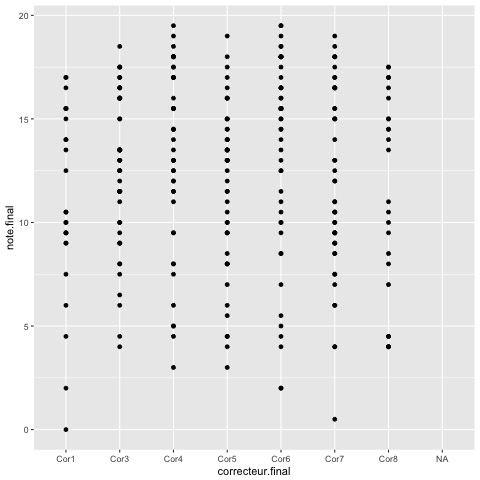
\includegraphics[width=70mm]{Figures/Notes/correcteur_final.jpg}
	\captionof{figure}{Scatterplot des notes de final en fonction des correcteurs}
	\label{fig:scatter_correcteur_final}
\end{center}


\section{Conclusion}
\end{document}
